\scanpage{9}\mspage{8}
I make explicit, because of its importance, the following property, although it will be a consequence in various ways of others

\deleted{\uline{At} DC 1 : Let $X,Y\in M$ with $\unsure{X|X'}\deleted{\unsure{\parallel}}\mathrel{\tikz[baseline=-.4ex,x=.65em,y=.65em]{\draw (0,1.1)--(1,.5)--(0,-.1) (1,1.1)--(0,.5)--(1,-.1);}}Y\unsure{\text{\S}|?|.}$}
\deleted{\deleted{\unsure{Then|At}} \inserted{Let} $X'\ll X$, \deleted{$Y'\ll Y\Longrightarrow X'\parallel\unsure{Y'|Y}$} \inserted{with $X'\parallel X\cap Y=L$, (i.e. $X'\parallel Z$ for $Z\leq X,Y$} $Y'\ll Y$ with $Y'\parallel L$. Then $X'\parallel Y'$}

% slanted
\margin{\uline{NB} The important thing is $X'\mathrel{\tikz[baseline=-.4ex,x=.65em,y=.65em]{\draw (0,1.1)--(1,.5)--(0,-.1) (1,1.1)--(0,.5)--(1,-.1);}}Y'$, then $X'\cap Y'=\unsure{\phi|\varnothing}$ immediate. For $Z\deleted{\ll}\leq X',\,Z\leq Y'$ $\Longrightarrow Z\ll X,\,Z\ll\unsure{Y'|Y}$ whence $Z\ll X\cap Y=L$, now $Z\leq X'\parallel L\underset{\mathrm{At}}{\Longrightarrow}Z\parallel L$, now $Z\ll L$ and $Z\parallel L$ this is \deleted{\unsure{impossible}} (\unsure{as|whence} $Z\mathrel{\tikz[baseline=-.4ex,x=.65em,y=.65em]{\draw (0,1.1)--(1,.5)--(0,-.1) (1,1.1)--(0,.5)--(1,-.1);}}L$) $\Longrightarrow Z^{+}\leq L$ \unsure{\deleted{absurd}|absurd} for \uline{$Z\cap L=\phi$ !}}%
% Connected thin upper, right-side and lower-oblique strokes crossing/bordering the NB note.
\margin{\tikz[x=.45em,y=.45em]{\draw (0,0)--(4,0);\draw (3.4,.2)--(3.6,-10);\draw (1.4,-6.4)--(3.9,-8.7);}}

\deleted{\uline{Corollary} 1 Let $F,C\in\mathscr F$ with $F\parallel C$. Then $F\ll F$, $C'\ll G\Longrightarrow F'\parallel G'$.}
\deleted{\uline{Corollary 2} Let $F,G\in\mathscr F$, $F\mathrel{\tikz[baseline=-.4ex,x=.65em,y=.65em]{\draw (0,1.1)--(1,.5)--(0,-.1) (1,1.1)--(0,.5)--(1,-.1);}}G$ \deleted{\unsure{with} $\unsure{L=\underset{Z\in\widetilde F\cap\widetilde G}{\mathrm{Sup}}\,Z}$} \inserted{$L=F\cap G$}, $F'\ll F,C'\ll G$. Suppose $F'\parallel L,\ C'\parallel L$, then $F'\parallel G'$.}

\deleted{\uline{At DC} 2 \quad (Axiom of \unsure{spacious|specious} workshops) \deleted{\unsure{Let|Let}} $X,Y\in M$, $\deleted{\unsure{L}}K=X\cap Y=\underset{Z\in\widetilde X\cap\widetilde Y}{\mathrm{Sup}}\,Z$. Suppose that for all $X',Y'$, with $X'\ll X,\underset{\tikz[x=1em,y=.35em,baseline=0pt]{\draw (0,0) .. controls (1,-.05) and (2,-.05) .. (3.4,.40);\draw (1.66,.16)--(1.85,.01)--(1.67,-.13);}}{Y'\ll Y,\ X'\parallel K},Y'\parallel K$, one has $X'\parallel Y'$. Then}

% Editing stroke beneath the preceding cancelled draft, with left oblique and rising right end.
\noindent\tikz[x=1em,y=1em]{\draw (0,.03) .. controls (2,.15) and (4,.18) .. (6,.12) .. controls (8,-.04) and (10,-.10) .. (11.1,-.08) .. controls (11.45,.55) and (11.55,.95) .. (12.2,1.18);\draw (-.18,-.03)--(.95,1.32);}

We shall want the

\uline{Property 1} Let $F,G\in\mathscr F$, $F\mathrel{\tikz[baseline=-.4ex,x=.65em,y=.65em]{\draw (0,1.1)--(1,.5)--(0,-.1) (1,1.1)--(0,.5)--(1,-.1);}}G$, $L=F\cap G$. Let $F'\ll F,\ G'\ll G$. Then
\[
\begin{aligned}
 & F'\mathrel{\tikz[baseline=-.4ex,x=.65em,y=.65em]{\draw (0,1.1)--(1,.5)--(0,-.1) (1,1.1)--(0,.5)--(1,-.1);}}G'\\
\Longleftrightarrow\quad & F'_{L}\mathrel{\tikz[baseline=-.4ex,x=.65em,y=.65em]{\draw (0,1.1)--(1,.5)--(0,-.1) (1,1.1)--(0,.5)--(1,-.1);}}G'_{L}
\end{aligned}
\]

cf \deleted{\unsure{page}} GF $\underline{\overline{\mathrm{VI}}}$, page~\uline{\unsure{73|13}} -- In any case we always have $\unsure{\mathrel{\tikz[x=.5em,y=.28em]{\draw (0,.08)--(1.2,.08) (0,.42)--(1.2,.42) .. controls (1.35,.42) and (1.38,.23) .. (1.28,.2);}}|\Rightarrow}$
\deleted{\unsure{Let us show} that we indeed have \unsure{in} $\Rightarrow$. Indeed,}

This is equivalent (if one views it in a general way) to the old At 12, which takes the name

% slanted
\margin{\uline{Criterion} of \uline{compatibility} for refinements of \uline{subfigures}\quad But this is false in the simplicial case, example :}%
\figure{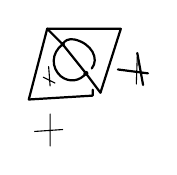
\begin{tikzpicture}[x=.035em,y=-.035em,line cap=round,line join=round]
\draw[thick] (30,10)--(106,10)--(85,76);
\draw[thick] (30,10)--(11,83)--(77,79)--(77,73);
\draw[thick] (30,10)--(46,26)--(70,56)--(85,76);
\draw[thick] (76,51) .. controls (84,41) and (76,25) .. (58,21)
 .. controls (52,20) and (48,22) .. (46,26)
 .. controls (34,35) and (34,50) .. (44,59)
 .. controls (53,66) and (64,64) .. (70,56);
\fill (46,26) circle (2.2) (70,56) circle (2.6);
\draw (26,60)--(38,66) (31.5,49)--(33,69);
\draw[thick] (103,52)--(134,56) (123,35)--(129,68);
\draw (123,39)--(122,67);
\draw (17,116)--(46,114) (33,98)--(33,131);
\end{tikzpicture}}
% slanted
\margin{But we shall have $X'_{L}\parallel Y'_{L}\Longrightarrow X'\mathrel{\tikz[x=.55em,y=.60em,line cap=round]{\draw (0,-.12)--(0,1) (.48,-.12)--(.48,1) (-.06,.30)--(.54,.47) (-.05,.51)--(.53,.65);}}Y'$, This is a counterexample to the : At $\unsure{\parallel|11}$, and a fortiori to \deleted{\unsure{ex}} At 11 (cf GF $\underline{\overline{\mathrm{VI}}}$, pages 67,68)}%

% Vertical rule bordering the axiom on its left.
\margin{\tikz[x=.5em,y=.5em]{\draw (0,0)--(0,4.25);}}
\uline{At DD} 1 Let \inserted{or else} $X,Y\ \&\ X',Y'\in M$, $X\mathrel{\tikz[baseline=-.4ex,x=.65em,y=.65em]{\draw (0,1.1)--(1,.5)--(0,-.1) (1,1.1)--(0,.5)--(1,-.1);}}Y,\ X'\ll X,Y'\ll Y$. Put $K=X\cap Y=\underset{Z\in\widetilde X\cap\widetilde Y}{\mathrm{Sup}}\,Z$. Then $X'_{L}\mathrel{\tikz[baseline=-.4ex,x=.65em,y=.65em]{\draw (0,1.1)--(1,.5)--(0,-.1) (1,1.1)--(0,.5)--(1,-.1);}}Y'_{L}$ implies $X'\mathrel{\tikz[baseline=-.4ex,x=.65em,y=.65em]{\draw (0,1.1)--(1,.5)--(0,-.1) (1,1.1)--(0,.5)--(1,-.1);}}Y'$ \quad (NB the converse \deleted{\unsure{is}} always true)

\uline{\unsure{Cor. Main|Corollary}} 1 \quad \unsure{the|the} ``property'' above

\[
F\parallel G,\ F'\ll F,\ C'\ll G\ \Longrightarrow\ F'\parallel G'
\tag*{\makebox[0pt][r]{\makebox[\displaywidth][l]{\uline{\unsure{Cor. Main|Corollary}} 2}}}
\]

More generally \quad If $F\mathrel{\tikz[baseline=-.4ex,x=.65em,y=.65em]{\draw (0,1.1)--(1,.5)--(0,-.1) (1,1.1)--(0,.5)--(1,-.1);}}G,\ F'\ll F,\ C'\ll G$, then
\[
 F'\parallel G'\ \Longleftrightarrow\ F'_{L}\parallel G'_{L}
\]
